\documentclass[12pt]{article}

\usepackage{sbc-template}
\usepackage{graphicx,url}
\usepackage[utf8]{inputenc}
\usepackage[english]{babel}
%\usepackage[latin1]{inputenc}  
\usepackage{xcolor}
\usepackage{cleveref}
\usepackage{listings}
%\usepackage{listings-golang} % import this package after listings

% ADD SUBSUBSUBSECTION
\newcommand{\subsubsubsection}[1]{\paragraph{#1}\mbox{}\\}
\setcounter{secnumdepth}{4}
\setcounter{tocdepth}{4}

%\lstset{ % add your own preferences
%    frame=single,
%    basicstyle=\footnotesize,
%    keywordstyle=\color{red},
%    numbers=left,
%    numbersep=5pt,
%    showstringspaces=false, 
%    stringstyle=\color{blue},
%    tabsize=4,
%    language=Golang % this is it !
%}
     
\sloppy

\title{Árion: A Blockchain Framework for Traceability in\\ Supply Chain Management}

\author{Edivaldo M. F. J. Júnior\inst{1}, Manoel C. M. Neto\inst{1}, Allan E. S. Freitas\inst{1}}


\address{Programa de Pós-Graduação em Engenharia de Sistemas e Produtos\\ Instituto Federal da Bahia (IFBA)\\ Campus de Salvador, 40301-015, Salvador -- BA -- Brazil
  \email{\{edivaldojunior,manoelnetom,allan\}@ifba.edu.br}
}

\begin{document} 

\maketitle

\begin{abstract}
A complex web of relationships provides goods for manufacturing, assembling, and delivering final products known as the supply chain. Emerging technologies have been used in supply chain systems in order to provide traceability. However, these systems tend to be centralized, monopolistic, and asymmetric. As a consequence, they may result in trusting problems, such as fraud, corruption, and tampering. Blockchain technology provides a new approach for information systems based on decentralization, that can apply for supply chain systems. This work presents a Blockchain-based framework for developing applications that provide such traceability for supply chain management. 
\end{abstract}

%\begin{keywords}
%Blockchain; supply chain management; traceability; smart contracts.
%\end{keywords}


\section{Introduction} \label{sec:Introduction}

Hundreds of years ago, supply chains were fairly simple. Mines and farms provided natural resources to skilled craftsman like blacksmiths and tailors who then created and sold goods. Nowadays, supply chains are much more complicated, fragmented and difficult to understand. 

Today's supply chains are so complex that even big industry players have difficulty tracking how their goods get made \cite{swan2015blockchain}. In order to solve some problems that come with this complexity, such as supply chain visibility and traceability, many systems have been developed. However, these systems typically store information in standard databases controlled by service providers. This centralized data storage becomes a single point of failure and risks tampering \cite{tian2017supply}.

Blockchain could make supply chain management simpler and more transparent. The idea is to create a single source of information about products and supply chain via global ledger. Each component would have its own entry on the blockchain that gets tracked over time. The end result is once the clients receive their products they could track every piece back to its manufacturer \cite{greve2018blockchain}.

This would reduce the need for large contract invoices on the back-and-forth of refund requests for faulty components. Those same smart contracts could assist with shipping and logistics tracking valuable products as they travel around the world. Using blockchain, companies can finally have a complete picture of their products at every stage in the supply chain, bringing transparency to the production process while reducing the cost of manufactured goods \cite{swan2015blockchain}.

This work presents Árion, a generic framework intended to be used in any kind of supply chain correlated to assets and products.
\section{Blockchain} \label{sec:Theoretical}

Blockchain can be considered as a public ledger, in which all committed transactions are stored in a block chain \cite{zheng2016blockchain}. For \cite{swan2015blockchain}, Blockchain is in a position to become the fifth disruptive computing paradigm after mainframes, PCs, Internet and mobile/ social networks. Blockchain technology has critical features, such as decentralization, persistence, anonymity and auditability. Also, Blockchain can function in a decentralized environment that is activated by the integration of several key technologies such as cryptographic hash, digital signature and distributed consensus engine, significantly save the cost and improve efficiency \cite{zheng2016blockchain}.

\subsection{Public Blockchain Versus Private Blockchain}\label{sec:versus}
On a public blockchain, any person can participate without a specific identity. They can be audited by anyone, and each node has as much transmission power as any other. For a transaction to be considered valid, it must be authorized by all nodes constituents via the consensus process. As long as each node meets protocol-specific stipulations, their transactions can be validated and thus added to the chain \cite{greve2018blockchain}. Private blockchains, on the other hand, perform a blockchain between a set of known and identified participants. A private blockchain provides a way to protect the interactions between a group of entities that have a common goal but that don't totally trust each other, like companies that trade funds, assets or information \cite{swan2015blockchain}.

%%%%%%%%%%%%%%%%%%%%%%%%%%%%%%%%%%%%%%%%%%%%%%
\subsection{Smart Contracts}\label{sec:smartContracts}
A smart contract is a computerized transaction protocol that executes the terms of a contract \cite{szabo1997idea}. The term smart contract (SC) means: “an internal transaction protocol format that executes the terms of a contract. Their overall goals are ensure common contractual conditions, minimize malicious and accidental exceptions and the need for reliable intermediaries. Related economic objectives include reducing fraud losses, arbitration and execution costs, and other transaction costs.” \cite{szabo1997idea}.

%%%%%%%%%%%%%%%%%%%%%%%%%%%%%%%%%%%%%%%%%%%%%%  
\section{Supply Chain Management} \label{sec:General}

There are billions of products being manufactured every day through complex supply chains that can extend to all parts of the world. However, tracing good flows from harvesting and manufacturing to the final consumer is hard \cite{galvez2018future}. Traceability is one of the key challenges encountered in the business world. Supply chain's transparency and end-to-end visibility can help shape product, raw material, test control, and end product flow\cite{tian2017supply}. Traceability systems typically store information in standard databases controlled by service providers. This centralized data storage becomes a single point of failure and tampering risks. As a consequence, these systems result in trusting problems, such as fraud, corruption, and tampering. Likewise, as a single point of failure, a centralized system is vulnerable to collapse \cite{tian2017supply}.

Nowadays, Blockchain presents a whole new approach based on decentralization, enabling end-to-end traceability, allowing consumers to access the asset's history of these products through a software application \cite{galvez2018future}. Supply chain management (SCM) requires to control who can write and read data to/from the Blockchain. In order to do that, the first step is identity. In the SCM context, the peers are known and the system needs to know who a user is, to define rules about what data they can commit, and what data they can consume from the ledger. So, in a corporate case scenario, Blockchain for the business, Blockchain for supply value chains, a private Blockchain provides this needed characteristic.
\section{Related Work} \label{sec:RelatedWork}
In order to solve some problems with Supply Chain traceability centralized, monopolistic, and asymmetric systems, many internet of things (IoT) technologies has been applied. However, these technologies do not guarantee that the information shared by supply chain members in the traceability systems can be trusted \cite{tian2017supply}.

In \cite{tian2017supply}, it is proposed a system that combines HACCP (Hazard Analysis and Critical Control Point, a food safety protocol), Blockchain and IoT in order to provide food safety traceability. Each supplu chain member can add, update and check the information about the product on the Blockchain as long as they register as a user in the system. Each product has also a unique digital cryptographic identifier that connects the physical items to their virtual identity in the system. This virtual identity can be seen as the product information profile.

The Everledger Diamonds project provides a Blockchain based solution to facilitate tracking from mine to consumer, enabling easier compliance against increasingly strict measures from diamonds produced \cite{crosby2016blockchain}.

These projects are focused on specific products only and are closed projects. Still, there is a general lack of standards for implementation of a Blockchain approach for traceability. A Blockchain must be universal and adaptable to specific situations \cite{valenta2017comparison}. In addition, the need to agree on a particular type of Blockchain to be used puts the parties under pressure. 

Our work is intended to provide a Blockchain based framework in order to facilitate the development of applications for traceability in supply chain management.
\section{Proposed Framework} \label{sec:Technical}
The main objective of this work is to create a generic framework for Supply Chain Management (SCM). Árion project is divided into three main modules described below: Frond-End WebApp, Back-End WebApp, and Data Storage. Figure~\ref{fig:detalhamentotecnico} shows the application architecture and its components. An SCM platform relies on three main items: assets, steps, and actors. Our approach is based on this triad, that must be defined on the creation of a new supply chain.

%htbp
\begin{figure}[ht]
\begin{center}
  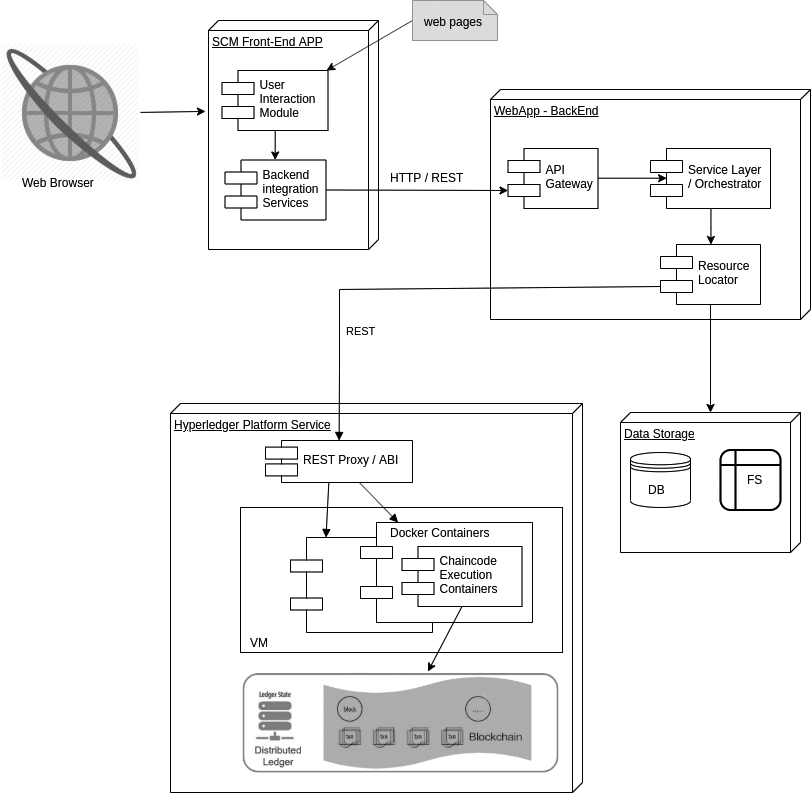
\includegraphics[scale=0.4]{images/detalhamentotecnico.png}
\caption{Árion Application architecture}
\label{fig:detalhamentotecnico}
\end{center}
\end{figure}

\subsection{Frond-End WebApp}\label{sec:WebAppFrondEnd}
Front-End WebApp is a client–server application which the client runs in a web browser. The Front-End Webapp is divided into two main blocks and these are classified according to the interactions: User Interaction Modules and Backend Interaction Services. User Interaction modules are responsible for providing web pages that will be rendered on client’s web browser. The backend interactions happen via a set of services.

\subsection{Back-End WebApp}\label{sec:WebAppBackEnd}
BackEnd - WebApp is a Middleware that runs on the server facilitating the client-server connectivity, forming a middle layer between the app and the network. It contains the logic to send the appropriate data back to the applicant. This module  is composed by the API Gateway, Service Layer and Resource Locator. API Gateway is a managed service that enables easily create, publish, maintain, monitor and secure REST APIs. The service Layer defines its set of available operations from the perspective of interfacing client layers. The service layer acts as an orchestrator, controlling the flow of incoming and outcoming information requests and responses. Resource locators are components that abstracts the persistence layer. Their job is to provide an object that can help services to discover and persist information from/to the Data Storage Module.

\subsection{Data Storage}\label{sec:DataStorage}
Árion uses three applications as data storage: Blockchain, Cloud file system, and relational database. Blockchains grow continuously because of the amount of data and code in them, which is unchanging. Therefore, an important design decision is to choose which data and calculations to keep in and out of the chain. A cloud file system is a tiered storage system that provides shared access to file data. A relational database is a set of formally described tables from which data can be accessed or reassembled in many different ways without having to reorganize the database tables. 

\subsubsection{Blockchain and Chaincode}\label{sec:DataStorageBlockchain}
The platform uses Blockchain to supply chain management tracking parts and service provenance, ensuring authenticity of goods, block counterfeits and reducing conflicts. This usually involves a limited and known number of actors, suggesting use of a permissioned Blockchain, that is, a Blockchain where all nodes must be allowed to be part of the system. To implement that, Hyperledger Fabric is used \cite{cachin2016architecture}. 

Hyperledger Fabric implements smart contracts through chaincode. In general, a smart contract defines the transaction logic that controls the lifecycle of a business object contained in the world state. It is then packaged into a chaincode which is then deployed to a Blockchain network. So, smart contracts rule transactions, whereas chaincode rules how smart contracts are packaged for deployment.

Before businesses transact with each other, they must define a common set of contracts covering common terms, data, rules, concept definitions, and processes. Taken together, these contracts lay out the business model that govern all of the interactions between transacting parties. A smart contract defines the rules between different organizations in executable code. Applications invoke a smart contract to generate transactions that are recorded on the ledger.


\section{Implementation Details} \label{sec:Implementation}
Our chaincode is written in Golang and provides all contracts needed to proceed traceability in our application. The first step is to create a JSON config file providing all information about these three items: the \textit{assetId}, a list of actors and a list of ordered steps. Our chaincode processes this file through  \textit{initLedger} and \textit{createNewAsset} functions. Front-end WebApp enables a user to define settings through a Configuration Page, adding these to the configuration file. 

Assets, asset items, steps and actors are described as \textit{structs}. Query methods are responsible for interact with the information of any item in the Blockchain. The function \textit{main} invokes the \textit{initLedger}, reads the configuration files and raises the platform enabling users to interact with the Blockchain via exposing its API. When creating an asset item, an \textit{AssetItemId} is generated. Each entity in the chain will have its unique entity ID and timestamp when it starts processing the transaction. By querying \textit{AssetItemId}, the user can easily track the current transaction information and status. Finally, completed all steps, the Blockchain will update \textit{deliverDate} and mark the status as completed once the final actor has received the order. \textit{ChangeAssetItemOwner} is the method called to update an asset item when it is moved from a step to another. It updates the \textit{CurrentOwnerId}, the \textit{ProcessDate}, information about prices and many other details of the transactions by the key/value map \textit{  aditionalInfo}. 

Figure~\ref{fig:sequenceDiagram} shows the interaction flow from users with Árion platform. Initially an admin persona creates and configure the SCM adding information about the steps and the users. After that, the admin can activate this SCM and from that point the actors can interact with the SCM to provide information about an asset item and also move this asset item through the supply chain. From that point too, any user can track an asset item to get information about the required good.

%htbp
\begin{figure}[ht]
\begin{center}
  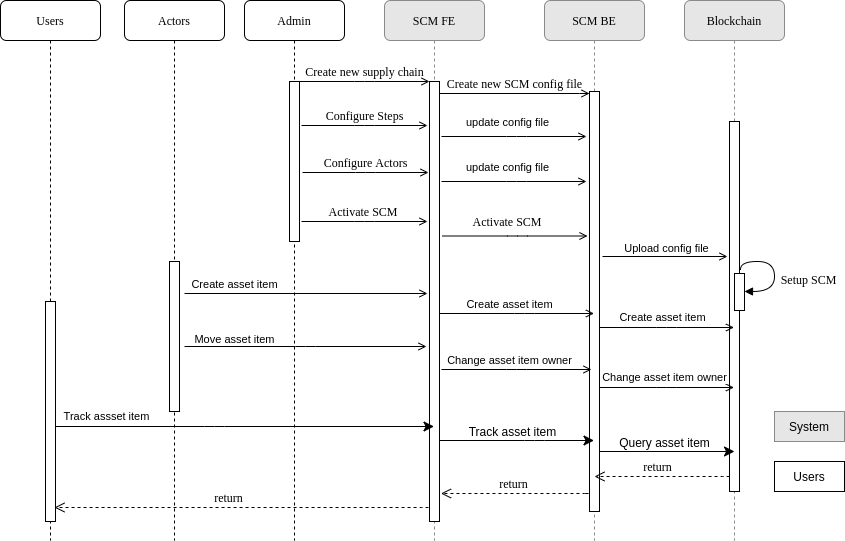
\includegraphics[scale=0.5]{images/SequenceDiagram.png}
\caption{SCM User flow}
\label{fig:sequenceDiagram}
\end{center}
\end{figure}
\section{Conclusion} \label{sec:Conclusion}

Although, some companies have launched pilot projects using Blockchain technology to manage their supply chains, no detailed information on the technical implementation of such projects has been reported. Either way, the retail industry has the potential to use this technology to improve traceability.  Even if some properties of Blockchain implementation may be useful for supply chain management, there are still a few uses to support this claim. 

In this paper, we proposed a framework for new decentralized traceability systems based on Blockchain technology. This system will deliver online information to all supply chain members on the safety status of goods, providing a more secure, distributed, transparent, and collaborative approach to supply chain management. The framework can significantly improve the development time of Supply Chain Management applications, and provide efficiency and transparency for product management on a supply chain. In a future work, we will present a proof of concept that exercises the use of proposed framework.

\bibliographystyle{sbc}
\bibliography{sbc-template}

\end{document}
